% !TEX encoding=utf8
\documentclass[10pt,a4paper]{scrartcl}

\usepackage{ucs}
\usepackage[utf8]{inputenc}
\usepackage[ngerman]{babel}
\usepackage{amsmath}
\usepackage{amssymb, amstext}
\usepackage{mathtools}
\usepackage[pdftex]{graphicx}
\usepackage{bibgerm}
\usepackage{amsthm}
\usepackage[colorlinks=true]{hyperref}
\usepackage{dsfont}
\usepackage{caption}
\usepackage{multicol}
\usepackage{pdfpages}
\usepackage{listings}
\usepackage[a4paper,left=2.5cm,right=2.5cm,top=2cm,bottom=4cm,bindingoffset=5mm]{geometry}
\usepackage{tikz}
%\usepackage{txfonts}
\usepackage{textcomp}
\usepackage{multirow}
\pagestyle{headings}
\usepackage{tabularx}
\usepackage{enumerate}
\newcolumntype{L}[1]{>{\raggedright\arraybackslash}p{#1}} % linksbündig mit Breitenangabe
\newcolumntype{C}[1]{>{\centering\arraybackslash}p{#1}} % zentriert mit Breitenangabe
\newcolumntype{R}[1]{>{\raggedleft\arraybackslash}p{#1}} % rechtsbündig mit Breitenangabe
\usepackage{subfig}

\setlength{\topmargin}{-15mm}
%\setcounter{secnumdepth}{5} %wie viele Level


%\usepackage[latin1]{inputenc}
\usepackage[T1]{fontenc}
%\usepackage{ae,aecompl}
%\usepackage{amsmath,amssymb,amstext}
\usepackage{psfrag}
\usepackage{caption}
\usepackage{booktabs}
\usepackage{tabularx}
\captionsetup[table]{textfont=it,justification=raggedright,singlelinecheck = false}
\usepackage{float}




%%%%

% einige Abkuerzungen
\newcommand{\C}{\mathbb{C}} % komplexe
\newcommand{\K}{\mathbb{K}} % komplexe
\newcommand{\R}{\mathbb{R}} % reelle
\newcommand{\Q}{\mathbb{Q}} % rationale
\newcommand{\Z}{\mathbb{Z}} % ganze
\newcommand{\N}{\mathbb{N}} % natuerliche

%Zum markieren: http://texwelt.de/wissen/fragen/2803/wie-kann-ich-formel-teile-einer-gleichung-einkreisen
\newcommand\mrahmen[3][]{%
  \tikz[anchor=base,baseline]\node[inner sep=2pt,draw=#2,#1]{$\displaystyle#3\mathstrut$};}
\colorlet{mfarbe}{red}


%verschiednen sachen die man mit begin{...} dann einzeln durchnummerrienen lassen kann
\newtheorem{defin}{Definition}
\newtheorem{satz}{Satz}
\newtheorem{formel}{Formel}
\newtheorem{abbildung}{Abbildung}
\newtheorem{versuch}{Versuch}


%Titel Gedöns
\title{Versuch F09\\ Neuromorphic Computing}
\date{Lab book}
\author{Xeno Boecker, Jan Jakob}
\date{}

\begin{document}


\pagenumbering{roman} %% small roman page numbers

%%% include the title
\thispagestyle{empty}  %% no header/footer (only) on this page
 \maketitle

%%% start a new page and display the table of contents
\newpage
\tableofcontents

%%% start a new page and display the list of figures
%\newpage
%\listoffigures

%%% start a new page and display the list of tables
%\newpage
%\listoftables

%%% display the main document on a new page 
\newpage

\pagenumbering{arabic} %% normal page numbers (include it, if roman was used above)


\section{Untersuchung eines einzelnen Neurons}

Im ersten Experiment untersuchen wir das Zündverhalten eines einzelnen Neurons ohne Input / äußere Stimuli. Das Neuron kann in einen kontinuierlichen Feuerzustand versetzt werden, wenn das Leck-Umkehrpotential die Zündschwelle übersteigt.

\subsection{Aufgabe 1}
Im Folgenden zeichnen wir ein Ersatzschaltbild eines Neurons in der beschriebenen Konfiguration. Dazu nehmen wir das Neuronenschema in Abbildung 5 als Referenz und stellen uns das Neuron als einen Kondensator vor, der an mehrere Spannungsquellen angeschlossen ist. Die verschiedenen Ionenkanäle der Nervenzelle werden zu einem
einem einzigen erregenden und einem einzigen hemmenden Potenzial zusammengefasst, und die Diffusion durch die Membran wird durch das Leckpotential ersetzt.

\begin{figure} [ht]
\begin{center}
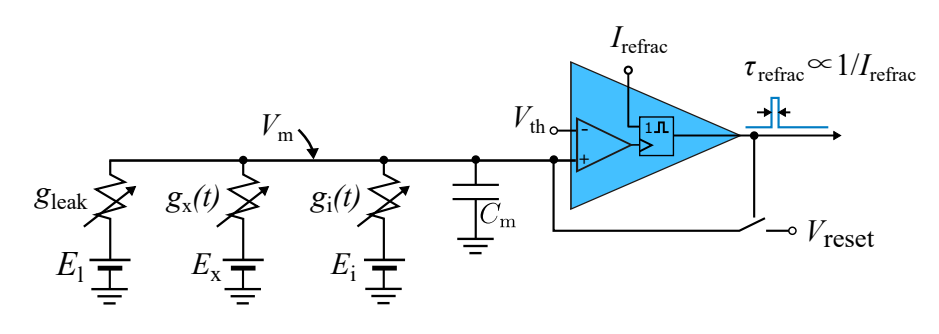
\includegraphics[scale=0.5]{pictures/Neuron_Circuit.png}
\caption{Ersatzschaltbild eines Neurons in der beschriebenen Konfigurationn}
\label{fig:schaltung1}
\end{center}
\end{figure}

\noindent \textbf{Frage:} Welche Parameter des Neurons beeinflussen die Feuerrate?

\begin{enumerate}
\item Refraktärzeit $\tau_{refrac}$
\item Membranzeitkonstante $\tau_m=\frac{C_m}{gl}$ 
\item Schwellwert- und Resetspannung $V_{th} , V_{reset}$
\end{enumerate}


\subsection{Aufgabe 2}
Bei dieser Aufgabe haben wir nur wie in der Versuchanleitung beschrieben Vorbereitungen getroffen und die aktuelle Shell für die Verwendung von Spikey eingerichtet.


\subsection{Aufgabe 3}
\noindent Auf dem Spikey-Chip wird ein einzelnes Neuron mit folgenden Parametern konfiguriert:

\begin{table}[H]
\centering
\captionsetup{justification=centering}
\caption{Parameter für ein einzelnes Neuron}
\begin{tabular}{l|l}
 Parameter&Wert\\
\hline
$V_{reset}$&$-80.0$mV\\
$E_{rev_I}$&$-75.0$mV\\
$V_{rest}$&$-50.0$mV\\
$V_{thresh}$&$-55.0$mV\\
$g_{leak}$&$20.0$
\end{tabular}
\label{tab:01}
\end{table}

\noindent Der Potentialverlauf ist in Abbildung \ref{fig:abb2} dargestellt. Wir lesen für die Werte $V_{reset}$ und $V_{th}$ folgende Werte ab:

\begin{table}[H]
\centering
\captionsetup{justification=centering}
\caption{Abgelesene Werte aus dem Verlauf des Membranpotentials}
\begin{tabular}{l|l}
 Parameter&Wert\\
\hline
$V_{reset}$&$-83.0 \pm 3.0$mV\\
$V_{thresh}$&$-56.0 \pm 3.0$mV
\end{tabular}
\label{tab:02}
\end{table}

\noindent Die Werte liegen jeweils im $3\sigma$-Bereich.
\begin{figure} [ht]
\begin{center}
\label{fig:abb2}
\caption{Verlauf des Membranpotentials}
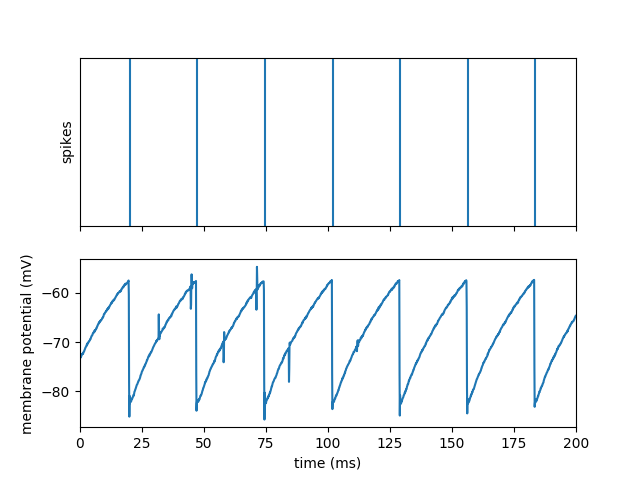
\includegraphics[scale=0.5]{experiments/SingleNeuron/fp_task1_1membrane.png} 
\end{center}
\end{figure}


\subsection{Aufgabe 4}
Durch Einsatz des Oszilloskops bestimmen wir die durchschnittliche Feuerrate des Neurons und ihre Standardabweichung mit Hilfe der Mess- und Statistikfunktion. Wir erhalten folgende Ergebnisse: 

\begin{align*}
f_{firing} = 355.4 \pm 3.4 kHz
\end{align*}

\begin{figure} [ht]
\begin{center}
\label{fig:abb3}
\caption{durchschnittliche Feuerrate durch Einsatz des Oszilloskops}
\includegraphics[scale=0.06]{pictures/oszilloskop_pic_1.jpg} 
\end{center}
\end{figure}

\noindent Wir berechnen die mittlere Feuerrate der im Spikes-Array empfangenen Spikes und vergleichen sie mit der Messung des Oszilloskops. Um eine Verteilung der Interspike-Intervalle (ISI) zu erhalten, berechnen wir die paarweise Differenz der empfangenen Spike-Zeiten und speichern sie in einem neuen Array. Den
Mittelwert dieser Differenzen und seine Standardabweichung berechnen wir mit den
entsprechenden NumPy-Funktionen.

\lstset{language=Python}
\lstset{frame=lines}
\lstset{caption={Berechnung der mittleren Feuerrate}}
\lstset{label={lst:code_direct}}
\lstset{basicstyle=\footnotesize}
\begin{lstlisting}
# time differences
timeDifferences = np.diff(spikes)

print("time differences mean", np.mean(timeDifferences))
print("time differences std deviation", np.std(timeDifferences))

print("firing rate mean", 1e4 / np.mean(timeDifferences))
print("firing rate std deviation", 1e4 / np.std(timeDifferences))
\end{lstlisting}
%\lstinputlisting[language=Python]{mesh.py}

\noindent Damit erhalten wir in Übereinstimmtung mit der obig bestimmten Feuerrate einen Wert von

\begin{align*}
f_{firing} = 356.5 \pm 4.7kHz.
\end{align*}

\noindent Den Faktor $1e4$ benötigen wir zur Umrechnung von biologischen Zeitskalen auf Chip-Zeitskalen.

\newpage


\section{Kalibrierung der Neuron-Parameter}
Durch Produktionsschwankungen bei der Herstellung des Chips kommt es zur sogenannten fixed pattern noise, was dazu führt, dass die Neuronen und die Synapsen-Parameter über den Chip variieren. Dies lässt sich durch Kalibrationsroutinen minimieren, was hier am Beispiel der Membranzeitkonstante $\tau_m$ durchgeführt wird. 

\subsection{Aufgabe 1}
Zunächst berechnen wir die theoretische Feuerrate aus den voreingestellten Werten. Nach Gleichung (6) aus der Versuchsanleitung gilt:
\begin{equation}
I_m(t)=C_m\frac{dV_m(t)}{dt}=g_l(E_l- V_m(t))
\end{equation} 
Nach Lösen der DGL erhält man:
\begin{equation}
V_m(t)=E_{leak} + (V_{res}-E_{leak})\cdot e^{-\frac{1}{\tau_m t}}
\end{equation}
Es soll nun 
\begin{equation}
V_m(t)=V_{thresh}
\end{equation}
gelten. Mit den Werten aus dem Pythonskript erhält man nach Umformen von (3) nach t einen Wert von:
\begin{equation*}
f_{firing}=-52.86 Hz
\end{equation*}
Die dabei verwendeten Werte für $V_{thresh}$ usw. entsprechen den in Versuchsteil 1 verwendeten Werten und können Tabelle 1 entnommen werden.


\subsection{Aufgabe 2}
Wir setzen den Schwellwert gerade auf den 1/e-ten Teil über $V_{reset}$, damit ist dieser nach $\tau_m$ erreicht. Eine Periode hat also gerade die Dauer $\tau_m + \tau_{refrac}$.
\begin{equation}
V_m(t = 1 / \tau_m) = V_{thresh} = E_{leak} + (V_{res}-E_{leak})\cdot e
\end{equation}
Stellen wir Gleichung (4) nach $V_{thresh}$, so erhalten wir
\begin{equation}
V_{thresh} = E_{leak} - 1/e\cdot (E_{leak} - V_{reset}),
\end{equation}
in Übereinstimmung mit Gleichung (8) aus der Versuchsanleitung. Mit den Parametern aus dem Skript ergibt sich ein neuer Wert von 
\begin{equation}
V_{thresh}=-51.69mV.
\end{equation}


\subsection{Aufgabe 3}
Wir ändern die Einstellung für $V_{thresh}$ im Skript entsprechend und führen das Skript aus. Außerdem stellen wir die Oszilloskop-Aufzeichnung so ein, dass alle 4 Membranspannungen zu sehen sind (Abbildung \ref{fig:abb4}). Wir verwenden die Messfunktionen des Oszilloskops, um gleichzeitig die Feuerfrequenz der vier angeschlossenen Neuronen zu messen. Außerdem aktivieren wir die Statistikfunktion, damit das Oszilloskop Mittelwerte und Standardabweichung berechnet. Wir erhalten folgende Werte:

\begin{figure} [ht]
\begin{center}
\label{fig:abb4}
\caption{Membranspannungen bei vier verschiedenen Neuronen}
\includegraphics[scale=0.04]{pictures/oszilloskop_pic_2.jpg} 
\end{center}
\end{figure}

\begin{table}[H]
\centering
\captionsetup{justification=centering}
\caption{Feuerrate der vier Neuronen}
\begin{tabular}{l|l}
 Neuron&Feuerrate\\
\hline
$1$&$377.4 \pm 36.8$kHz\\
$2$&$343.8 \pm 39.6$kHz\\
$3$&$446.7 \pm 24.8$kHz\\
$4$&$218.8 \pm 73.9$kHz
\end{tabular}
\label{tab:01}
\end{table}

\newpage


\subsection{Aufgabe 4}
Über die Variation der Leitfähigkeiten $g_{leak}$ kann die Feuerrate verändert werden. Wir kalibrieren die 4 Neuronen für eine identische Feuerrate und damit identische Membranzeitkonstante, indem wir einen neuen Leckleitwert $g_{leak}'$ für jedes Neuron einstellen. Zur Berechnung von $g_{leak}'$ verwenden wir folgende Überlegung:
\begin{align*}
f_{firing}&=g_{leak}/C_m\\f_{firing}‘&=g_{leak}/C_m*1/g_{leak}*g_{leak}’\\&=f_{firing}/g_{leak}*g_{leak}’\\g_{leak}’&=f_{firing}‘/f_{firing}*g_{leak}
\end{align*}

\noindent Setzen wir die entsprechenden Werte ein, so erhalten wir:

\begin{table}[H]
\centering
\captionsetup{justification=centering}
\caption{Neue $g_{leak}'$ Werte der vier Neuronen}
\begin{tabular}{l|l}
 Neuron&$g_{leak}'$\\
\hline
$1$&$145.6 nS$\\
$2$&$90.8 nS$\\
$3$&$115.1 nS$\\
$4$&$107.5 nS$
\end{tabular}
\label{tab:01}
\end{table}

\noindent Die Schwankungen kommen von Herstellungsungenauigkeiten (fixed pattern noise). Zudem ist uns aufgefallen, dass es eine gewisse trial to trial Variabilität gab (durch elektrisches und thermisches Rauschen). 


\subsection{Aufgabe 5}
Wie man sehen kann, erhält man eine asymmetrische Verteilung, die poissonartig aussieht. Dies ist in sehr guter Übereinstimmung mit dem Histrogramm aus der Versuchsanleitung.


\begin{figure} [ht]
\begin{center}
\label{fig:abb4}
\caption{Histogramm der Membranzeitkonstanten von 192 unkalibrierten Neuronen}
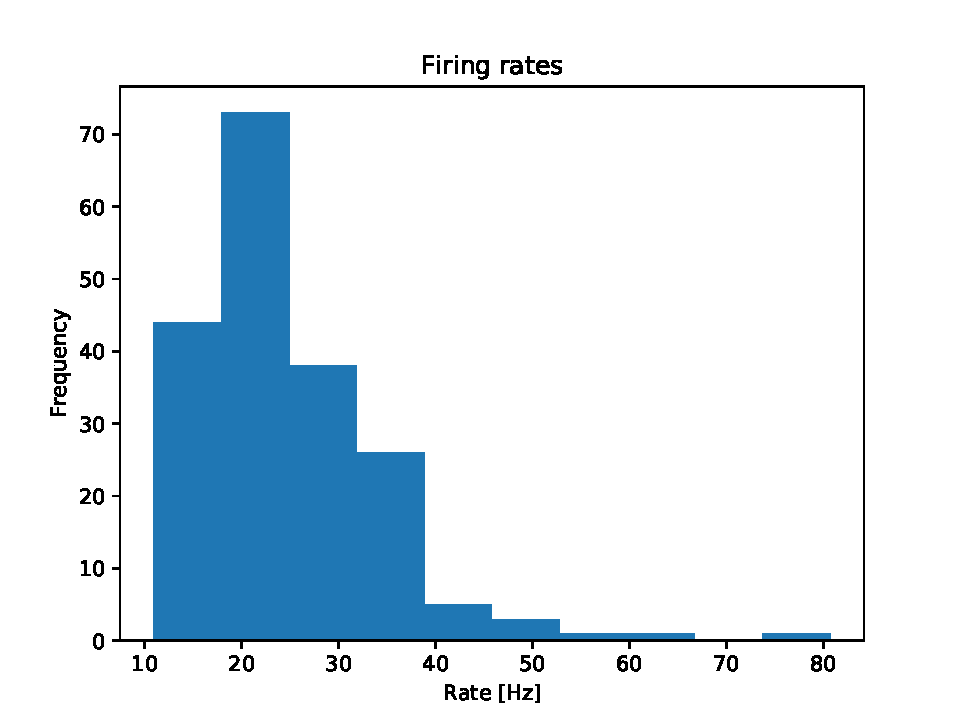
\includegraphics[scale=0.35]{pictures/firing_rates.pdf} 
\end{center}
\end{figure}


\newpage


\section{Einzelnes Neuron mit synaptischem Input}
In dieser Aufgabe bewerten wir den Einfluss des synaptischen Inputs auf das Neuron.


\subsection{Aufgabe 1}
Die Parameter drvifall und drviout werden variiert, dabei wird beobachtet, dass die EPSP-Kurve für kleine Werte von drvifall schneller abfällt und der Peak wird größer. Für kleinere Werte von drviout wird der Peak hingegen leicht kleiner und die EPSP-Kurve fällt minimal langsamer ab.

\begin{figure} [ht]
\begin{center}
\label{fig:abb6}
\caption{EPSP mit Parametern drvifall=1.5, drviout=1.6}
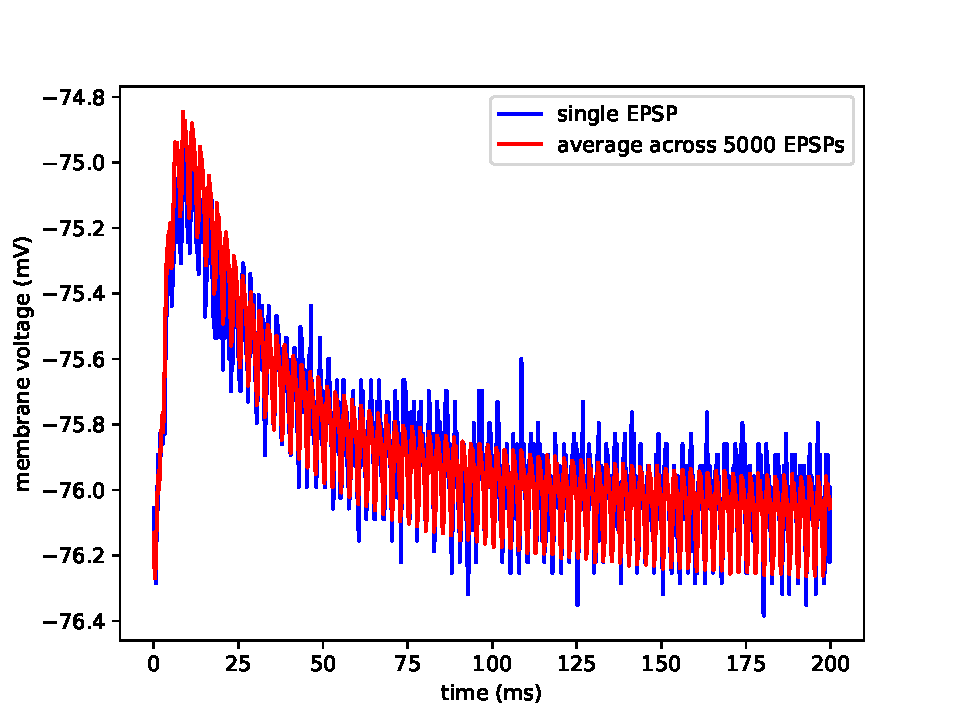
\includegraphics[scale=0.35]{pictures/epsp_fall_1_5_out_1_6.pdf} 
\end{center}
\end{figure}

\begin{figure} [ht]
\begin{center}
\label{fig:abb7}
\caption{EPSP mit Parametern drvifall=0.1, drviout=1.6}
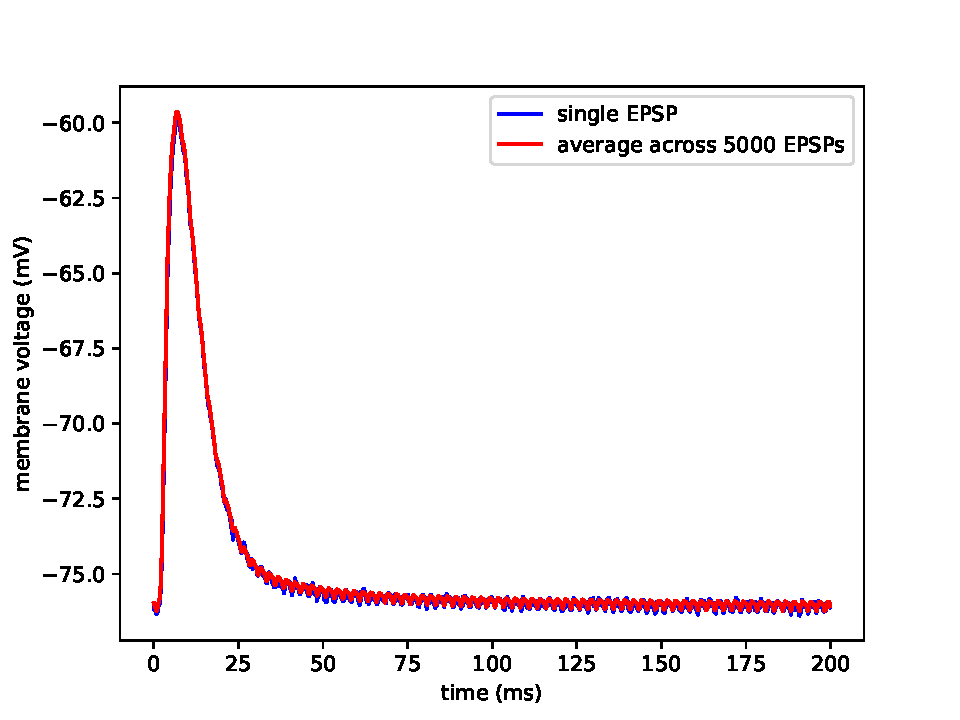
\includegraphics[scale=0.35]{pictures/epsp_fall_0_1_out_1_6.pdf} 
\end{center}
\end{figure}

\begin{figure} [ht]
\begin{center}
\label{fig:abb8}
\caption{EPSP mit Parametern drvifall=1.5, drviout=0.3}
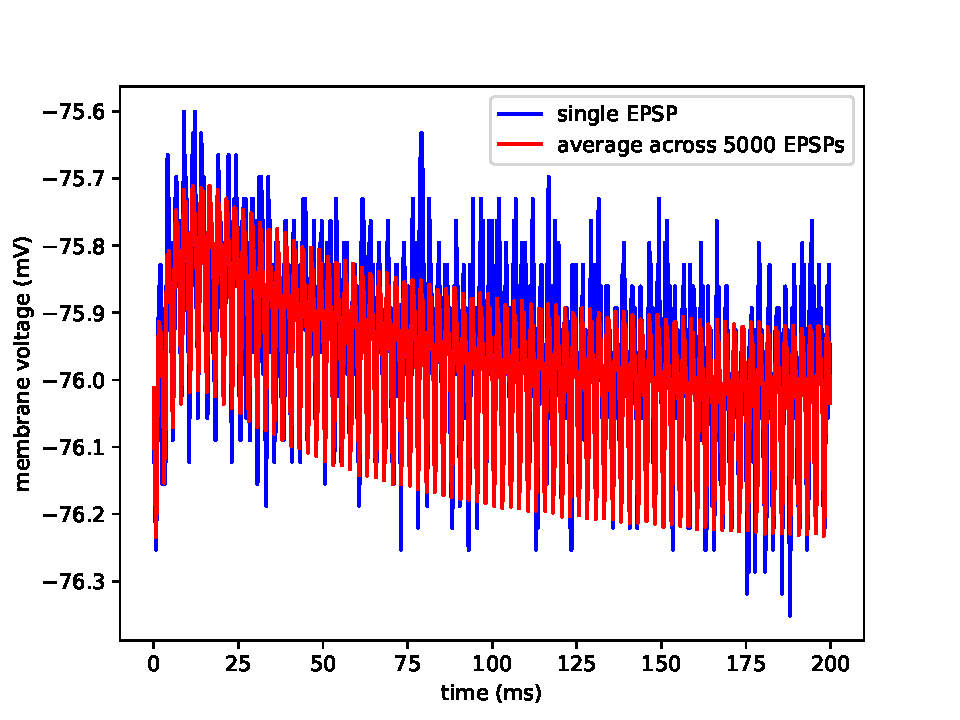
\includegraphics[scale=0.35]{pictures/epsp_fall_1_5_out_0_3.pdf} 
\end{center}
\end{figure}


\subsection{Aufgabe 2}
Wie erwartet ist der Peak umgekehrt. Das Verhalten der beiden Parameter drvifall und drviout ist hingegen unverändert im Vergleich zum EPSP.


\begin{figure} [ht]
\begin{center}
\label{fig:abb9}
\caption{IPSP mit Parametern drvifall=1.5, drviout=1.6}
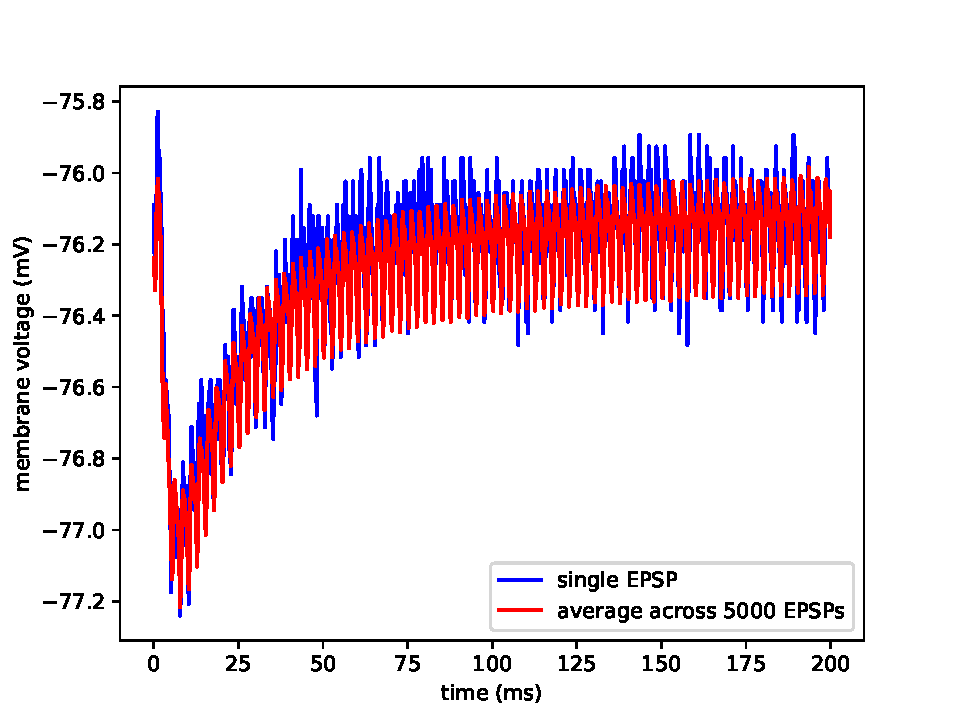
\includegraphics[scale=0.35]{pictures/epsp_inhibitory_fall_1_5_out_1_6.pdf} 
\end{center}
\end{figure}


\subsection{Aufgabe 3}
Wir untersuchen das fixed-pattern noise zwischen verschiedenen Synapsen. Hierzu werden von 192 Synapsen gemittelte EPSP-Läufe aufgenommen und deren Höhe bestimmt. Die Verteilung ist als Histogramm in Abbildung \ref{fig:abb10} zu sehen. Die berechnete Varianz der EPSP-Höhen beträgt $\sigma^2= 23.14mV^2$.

\begin{figure} [ht]
\begin{center}
\label{fig:abb10}
\caption{Histogramm der EPSP-Höhen von 192 Synapsen}
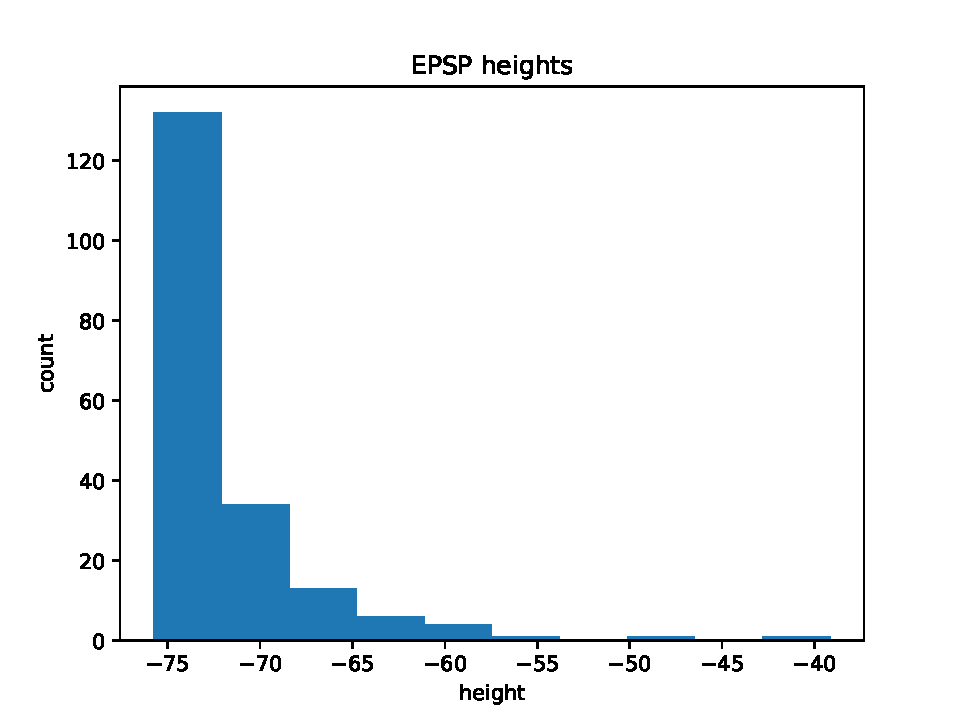
\includegraphics[scale=0.35]{pictures/epsp_heights.pdf} 
\end{center}
\end{figure}


\subsection{Aufgabe 4}
Wir verwenden eine andere Stimuluserzeugung zur Beobachtung gestapelter
EPSPs und reduzieren den zeitlichen Abstand zwischen den Eingangs-Spikes
bis das Neuron mindestens einmal feuert. In einem festen Zeitabstand werden Input-Spikes erzeugt, bis die Summe der Potentiale den Schwellwert (Threshold) übersteigt und das Neuron feuert. Ist der Zeitabstand zwischen zwei Input-Spikes zu groß, so kommt es zu keiner zeitlichen Summation der Signale.\\

\noindent Vergleich der relativen Höhen der verschiedenen PSPs qualitativ mit den vorherigen Ergebnissen des fixed-pattern noise: Der Peak des Membranpotentials hat einen höheren Wert wie die resultierenden PSP-Höhen in Aufgabe 3. Dies liegt daran, dass die Eingangs-Spikes gestapelt werden. Unterschiedliche Peak-Höhen zeigen außerdem das fixed pattern noise sehr deutlich.

\begin{figure} [ht]
\begin{center}
\label{fig:abb10}
\caption{Anregungen durch verschiedene Synapsen. Unterschiedliche Peak-Höhen zeigen das fixed pattern noise sehr deutlich.}
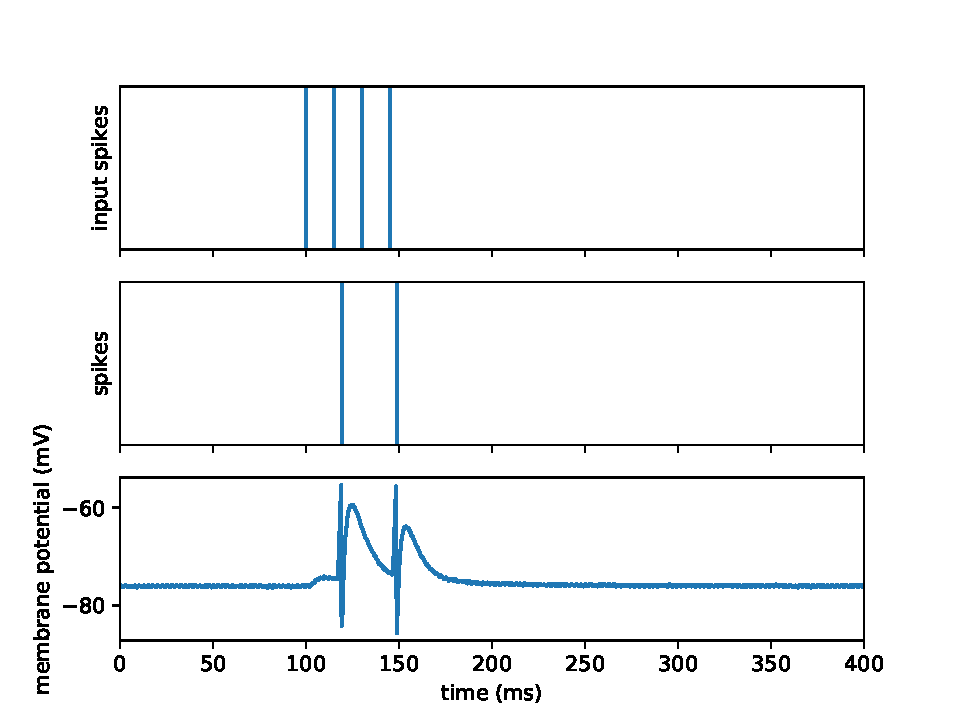
\includegraphics[scale=0.5]{pictures/resonant_firing.pdf} 
\end{center}
\end{figure}


\newpage


\section{Kurzzeit-Plastizität}
In dieser Aufgabe untersuchen wir die Hardware-Implementierung der Kurzzeitplastizität (STP). 

\subsection{Aufgabe 1}
Wir starten mit dem depressing mode ($\tau_{fac} = 0$). Wir beobachten folgendes Verhalten:
\begin{itemize}
\item Verkleinert man die die spike distance, desto schneller erfolgt der Abfall des ersten Peaks zu einem stationären Plateau und je keiner die spike distance, desto größer der Wert dieses Plateaus. Dieses Verhalten liegt nahe, wurde aber nicht beobachtet, da wir anfänglich $\tau_{rec}$ zu klein gewählt haben. Hier spielen zwei konträre Effekte eine Rolle: Durch eine kürzere spiking distance ist zwar jeder einzelne Peak kleiner (da stärker unterdrückt), aber durch Summation ist das Gesamtpotential wieder größer.
\item Je größer die final spike distance, desto größer ist der letzte Peak (weniger stark depressed).
\item Vergrößert man die Utilization $U$ so werden die Werte der PSP-Höhen größer und fallen schneller ab.
\item Umso größer man $\tau_{rec}$ wählt, desto stärker wird der letzte Peak unterdrückt und desto schneller fällt die Amplitude auf den stationären Fall ab.
\end{itemize} 

\begin{figure} [ht]
\begin{center}
\label{fig:abb11}
\caption{spike distance: 50.0ms, final spike distance: 100.0ms}
\includegraphics[scale=0.35]{pictures/final_spike_variation_1.pdf} 
\end{center}
\end{figure}

\newpage

\begin{figure} [ht]
\begin{center}
\label{fig:abb12}
\caption{spike distance: 100.0ms, final spike distance: 300.0ms}
\includegraphics[scale=0.35]{pictures/final_spike_variation_2.pdf} 
\end{center}
\end{figure}

\begin{figure} [ht]
\begin{center}
\label{fig:abb13}
\caption{spike distance: 10.0ms, final spike distance: 300.0ms}
\includegraphics[scale=0.35]{pictures/final_spike_variation_3.pdf} 
\end{center}
\end{figure}

\begin{figure} [ht]
\begin{center}
\label{fig:abb14}
\caption{spike distance: 100.0ms, final spike distance: 100.0ms}
\includegraphics[scale=0.35]{pictures/final_spike_variation_4.pdf} 
\end{center}
\end{figure}

\newpage

\begin{figure} [ht]
\begin{center}
\label{fig:abb15}
\caption{spike distance: 100.0ms, final spike distance: 200.0ms}
\includegraphics[scale=0.35]{pictures/final_spike_variation_5.pdf} 
\end{center}
\end{figure}


\begin{figure} [ht]
\begin{center}
\label{fig:abb16}
\caption{spike distance: 100.0ms, final spike distance: 500.0ms}
\includegraphics[scale=0.35]{pictures/final_spike_variation_6.pdf} 
\end{center}
\end{figure}

\begin{figure} [ht]
\begin{center}
\label{fig:abb17}
\caption{U: 0.2, spike distance: 100.0ms, final spike distance: 150.0ms}
\includegraphics[scale=0.35]{pictures/final_spike_variation_7.pdf} 
\end{center}
\end{figure}

\newpage

\begin{figure} [ht]
\begin{center}
\label{fig:abb18}
\caption{U: 0.8, spike distance: 100.0ms, final spike distance: 150.0ms}
\includegraphics[scale=0.35]{pictures/final_spike_variation_8.pdf} 
\end{center}
\end{figure}

\begin{figure} [ht]
\begin{center}
\label{fig:abb19}
\caption{$\tau_{rec}$: 100.0ms, final spike distance: 200.0ms, U: 0.6, spike distance: 100.0ms}
\includegraphics[scale=0.35]{pictures/final_spike_variation_9.pdf} 
\end{center}
\end{figure}

\begin{figure} [ht]
\begin{center}
\label{fig:abb20}
\caption{$\tau_{rec}$: 150.0ms, final spike distance: 200.0ms, U: 0.6, spike distance: 100.0ms}
\includegraphics[scale=0.35]{pictures/final_spike_variation_10.pdf} 
\end{center}
\end{figure}

\newpage

\begin{figure} [ht]
\begin{center}
\label{fig:abb21}
\caption{$\tau_{rec}$: 200.0ms, final spike distance: 200.0ms, U: 0.6, spike distance: 100.0ms}
\includegraphics[scale=0.35]{pictures/final_spike_variation_11.pdf} 
\end{center}
\end{figure}


\subsection{Aufgabe 2}
Wird STP deaktiviert, so ist der erste Peak kleiner als die nachfolgenden.


\subsection{Aufgabe 3}
Wir schalten in den falilating mode ($\tau_{rec} = 0$) und untersuchen analog das Verhalten des Membranpotentials. Wir beobachten folgendes Verhalten:
\begin{itemize}
\item Verringert man die spike distance, so erhält man durch Summation der einzelnen Peaks einen höheren Wert für die Peaks des Membranpotentials.
\item Je kleiner die final spike distance, desto größer ist der letzte Peak, da er noch stärker begünstigt wird.
\item Verkleinert man die Utilization $U$, so werden die Werte der PSP-Höhen größer und fallen schneller ab.
\item Umso größer man $\tau_{fac}$ wählt, desto stärker wird der letzte Peak verstärkt.
\end{itemize} 

\begin{figure} [ht]
\begin{center}
\label{fig:abb22}
\caption{spike distance: 300.0ms, $\tau_{fac}$: 100.0ms, U: 0.8, final spike distance: 300.0ms}
\includegraphics[scale=0.35]{pictures/final_spike_variation_12.pdf} 
\end{center}
\end{figure}

\newpage

\begin{figure} [ht]
\begin{center}
\label{fig:abb23}
\caption{spike distance: 100.0ms, $\tau_{fac}$: 100.0ms, U: 0.8, final spike distance: 300.0ms}
\includegraphics[scale=0.35]{pictures/final_spike_variation_13.pdf} 
\end{center}
\end{figure}

\begin{figure} [ht]
\begin{center}
\label{fig:abb24}
\caption{final spike distance: 100.0ms, $\tau_{fac}$, 150.0, U: 0.6, spike distance: 100.0ms}
\includegraphics[scale=0.35]{pictures/final_spike_variation_14.pdf} 
\end{center}
\end{figure}

\begin{figure} [ht]
\begin{center}
\label{fig:abb25}
\caption{final spike distance: 300.0ms, $\tau_{fac}$: 150.0ms, U: 0.6, spike distance: 100.0ms}
\includegraphics[scale=0.35]{pictures/final_spike_variation_15.pdf} 
\end{center}
\end{figure}

\newpage

\begin{figure} [ht]
\begin{center}
\label{fig:abb26}
\caption{final spike distance: 500.0ms, $\tau_{fac}$: 150.0ms, U: 0.6, spike distance: 100.0ms}
\includegraphics[scale=0.35]{pictures/final_spike_variation_16.pdf} 
\end{center}
\end{figure}

\begin{figure} [ht]
\begin{center}
\label{fig:abb27}
\caption{U: 0.4, $\tau_{fac}$: 100.0ms, spike distance: 100.0ms, final spike distance: 300.0ms}
\includegraphics[scale=0.35]{pictures/final_spike_variation_17.pdf} 
\end{center}
\end{figure}

\begin{figure} [ht]
\begin{center}
\label{fig:abb28}
\caption{U: 0.8, $\tau_{fac}$: 100.0ms, spike distance: 100.0ms, final spike distance: 300.0ms}
\includegraphics[scale=0.35]{pictures/final_spike_variation_18.pdf} 
\end{center}
\end{figure}

\newpage

\begin{figure} [ht]
\begin{center}
\label{fig:abb29}
\caption{$\tau_{fac}$: 50.0ms, U: 0.6, spike distance: 100.0ms, final spike distance: 300.0ms}
\includegraphics[scale=0.35]{pictures/final_spike_variation_19.pdf} 
\end{center}
\end{figure}

\begin{figure} [ht]
\begin{center}
\label{fig:abb30}
\caption{$\tau_{fac}$: 200.0ms, U: 0.6, spike distance: 100.0ms, final spike distance: 300.0ms}
\includegraphics[scale=0.35]{pictures/final_spike_variation_20.pdf} 
\end{center}
\end{figure}


\newpage


\section{Feed-Forward Netzwerke}
Wir untersuchen ein neuronales Netz am Beispiel einer vorwärts gerichteten Synfire Chain. Der Aufbau erfolgt gemäß Abbildung \ref{fig:abb11100}. Die Kettenglieder sind Populationen und bestehen aus einer gewissen Anzahl an Neuronen. Jede Population ist jeweils mit der nächsten Population verbunden. Eine Gruppe (Spalte) feuert dabei immer synchron. Die inhibitorischen Neuronen verhindern ein Doppelfeuern der exzitatorischen. 

\begin{figure} [ht]
\begin{center}
\label{fig:abb4}
\caption{Schematische Darstellung einer Synfire-Kette mit Feed-Forward-Hemmung. Erregende und hemmende Neuronen sind rot bzw. blau gefärbt}
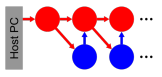
\includegraphics[scale=0.8]{pictures/synfire_chain.png}
\end{center}
\end{figure}

\subsection{Aufgabe 1}
Das Feuerverhalten der Synfire-Chain hängt maßgeblich von den synaptischen Gewichten ab. Um das in Abbildung \ref{fig:abb10} dargestellte Verhalten zu produzieren, haben wir folgende Gewichte verwendet:

\begin{table}[H]
\centering
\captionsetup{justification=centering}
\caption{Verbindungsgewichte Synfire-Chain}
\begin{tabular}{l|l}
 Gewicht&Wert\\
\hline
StimExcExc&2 $\cdot$ pynn.minExcWeight()\\
StimExcInh&2 $\cdot$ pynn.minExcWeight()\\
ExcExc&2 $\cdot$ pynn.minExcWeight()\\
ExcInh&1 $\cdot$ pynn.minExcWeight()\\
InhExc&15 $\cdot$ pynn.minInhWeight()
\end{tabular}
\label{tab:05}
\end{table}

\noindent Die exc-exc scheint die sensitivste Verbindung zu sein, da hier kleine Veränderungen des Gewichts einen sehr hohen Einfluss auf das Feuerverhalten der Synfire-Chain hatten. Die inhibitorischen Neuronen kann man mit folgenden Gewichtseinstellungen deaktivieren:

\begin{table}[H]
\centering
\captionsetup{justification=centering}
\caption{Verbindungsgewichte bei deaktivierter Inhibition}
\begin{tabular}{l|l}
 Gewicht&Wert\\
\hline
StimExcExc&2 $\cdot$ pynn.minExcWeight()\\
StimExcInh&0 $\cdot$ pynn.minExcWeight()\\
ExcExc&2 $\cdot$ pynn.minExcWeight()\\
ExcInh&0 $\cdot$ pynn.minExcWeight()\\
InhExc&0 $\cdot$ pynn.minInhWeight()
\end{tabular}
\label{tab:06}
\end{table}

\noindent Mit diesen Gewichten erhält man das in Abbildung \ref{fig:abb10} dargestellte Verhalten. Man sieht, das die Hälfte aller Neuronen nun nicht mehr feuert sowie eine Auffächerung: Eine größere Anzahl an Neuronen feuert nun mehrfach.

\begin{figure} [ht]
\begin{center}
\label{fig:abb4}
\caption{Aktivität der Synfire-Kette einschließlich des Membranpotenzials des Neurons mit ID=0}
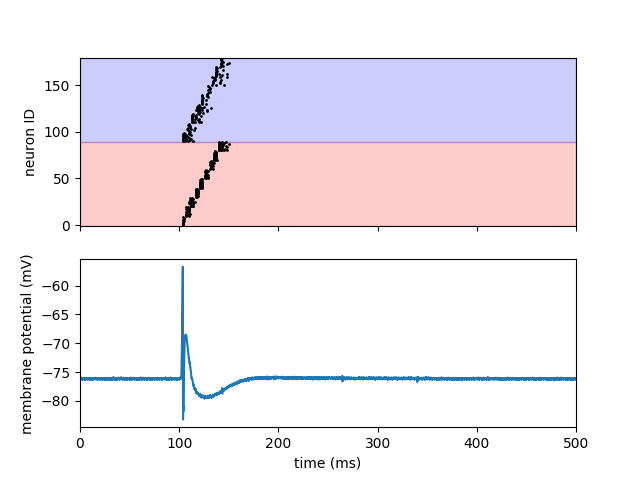
\includegraphics[scale=0.35]{pictures/task1_synfire_chain.png}
\end{center}
\end{figure}

\begin{figure} [ht]
\begin{center}
\label{fig:abb4}
\caption{Aktivität der Synfire-Kette mit deaktivierter Inhibition}
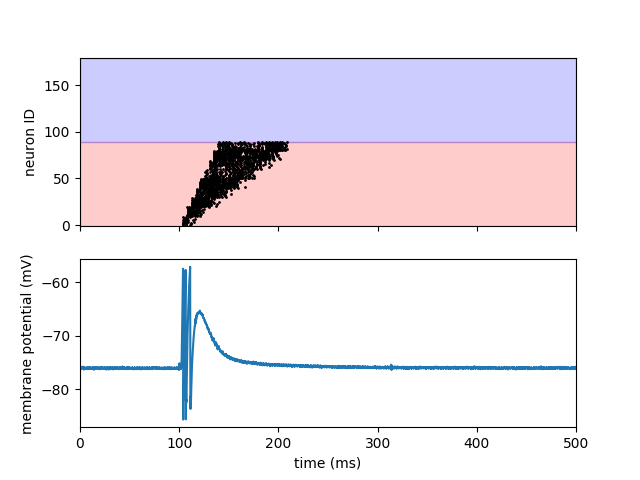
\includegraphics[scale=0.35]{pictures/synfire_chain_disable_inhibition.png}
\end{center}
\end{figure}


\newpage 


\subsection{Aufgabe 2}
Mit einer kleineren Anzahl an Neuronen je Population kann die Kettenlänge und die Dauer der Netzwerkaktivität erhöht werden.
maximal chain length: 2exc, 1inh --> length: 64 populations
Which hardware feature limits the min nbr of neurons in each population --> lukas
What is the maximal chain length that you can produce?


\begin{figure} [ht]
\begin{center}
\label{fig:abb4}
\caption{df}
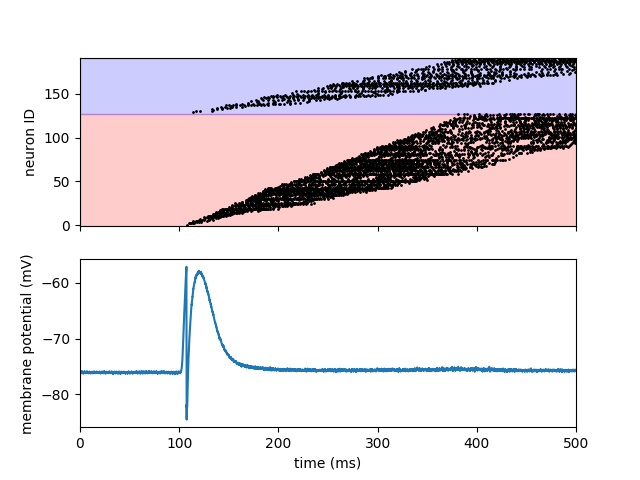
\includegraphics[scale=0.35]{pictures/chainlength_64.png}
\end{center}
\end{figure}

Die starke Auffächerung der Kette lässt sich durch die starke 
\subsection{Aufgabe 3}
Wir schließen die Synfire-Chain, indem wir die letzte Population an Neuronen mit der ersten verbinden.
\begin{figure} [ht]
\begin{center}
\label{fig:abb4}
\caption{Aktivität der Synfire-Kette mit in einer Loop-Konfiguration, in der die letzte Population die erste stimuliert}
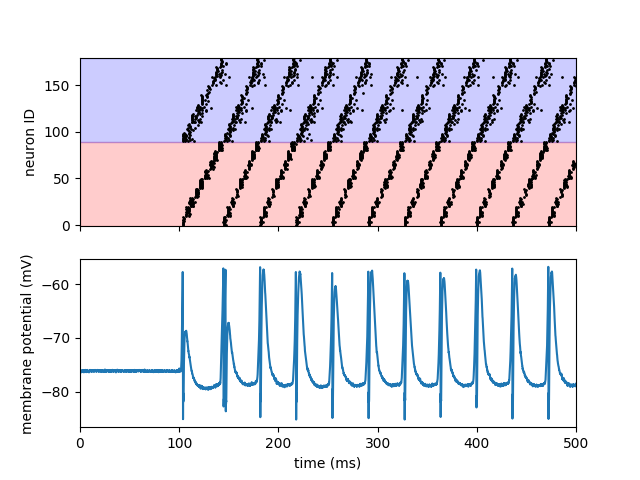
\includegraphics[scale=0.35]{pictures/synfire_chain_loop.png}
\end{center}
\end{figure}

Record 4 hardware neurons on the oszi from ascending populations (see the temporal difference):
ecord 4 hardware neurons on the oscilloscope from ascending populations to see the
temporal difference of the arriving PSPs on the membranes and observe the timing of
the arriving excitatory stimulus and the feed-forward inhibition. Convince yourself that
the activity is sustained even after the software run completed.


\begin{figure} [ht]
\begin{center}
\label{fig:abb4}
\caption{Aktivität der Synfire-Kette mit abgestellter Inhibition einschließlich des Membranpotenzials des Neurons mit ID=0}
\includegraphics[scale=0.05]{pictures/oszilloskop_pic_3.jpg}
\end{center}
\end{figure}

\newpage


\section{Rekurrente Netzwerke}
What would happen if we would want to use excitatory connections? --> Lukas
For each neuron, measure the firing rate and plot it against the
CVs of inter-spike intervals

Wir versetzen eine Population von einigen Neuronen in einen kontinuierlich feuernden Zustand. 

\subsection{Aufgabe 1}
\begin{figure} [ht]
\begin{center}
\label{fig:abb4}
\caption{Feuerrate in Abhängigkeit der CVs}
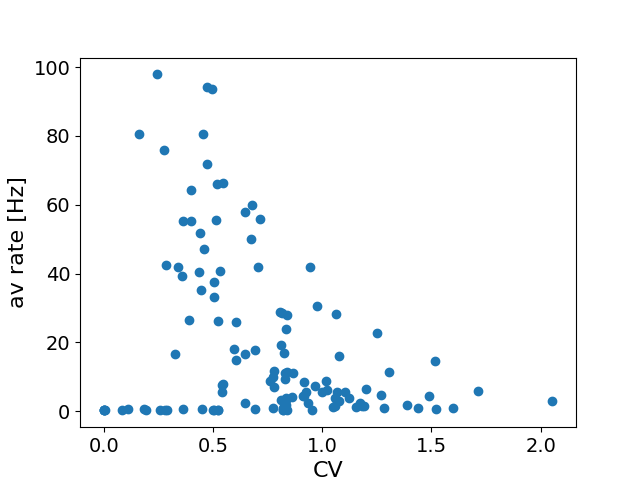
\includegraphics[scale=0.45]{pictures/decorr_rate_over_cv.png}
\end{center}
\end{figure}

Interpret the correlation between firing rates and CVs:
CV größer --> rate kleiner
größere Abweichungen, dann wird manchmal der Threshold nicht überschritten und die chain bricht ab.



\subsection{Aufgabe 2}

\begin{figure} [ht]
\begin{center}
\label{fig:abb4}
\caption{Feuerrate in Abhängigkeit der CVs}
\includegraphics[scale=0.45]{pictures/CVs.pdf}
\end{center}
\end{figure}

\begin{figure} [ht]
\begin{center}
\label{fig:abb4}
\caption{Feuerrate in Abhängigkeit der CVs}
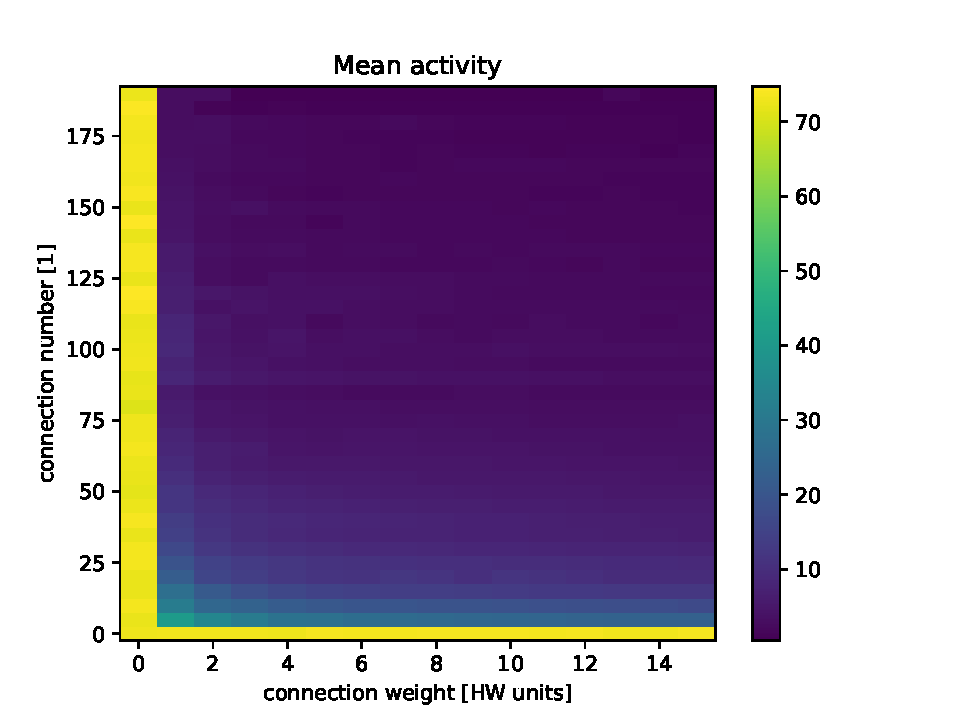
\includegraphics[scale=0.45]{pictures/mean_activity.pdf}
\end{center}
\end{figure}


\subsection{Aufgabe 3}
Im letzten Teil des Versuchs wurde versucht die Feuerraten auf 25 Hz zu bringen. Das haben wir mit einem Gewicht von 1 und 23 Verbindungen am besten geschafft (25.1 Hz). Die Job Id war: job 150194 (leider haben wir die Daten nicht mehr, da der Job gelöscht wurde und nicht in der letzten jupyter Version war, die wir heruntergeladen haben), sonst hätten wir auch noch die verschiedenen Plots dazu abgespeichert. 
 
Calibrate the network towards a firing rate of approximately 25 Hz. Write down the
used parameters and save the results. Optional: Try to maximize the average CV, while
keeping the firing rate constant.

calibrate network to 25Hz
Parameters used:
w = 2, k = 10
--> 24.8 Hz


\newpage


\section{Eine einfache Berechnung - XOR}


\subsection{Aufgabe 1}
Assume that everything works perfectly (i.e. all neurons work and each input spike
triggers exactly one output spike). Can you come up with a smaller network that can
perform this task, given that each neuron can only have either excitatory or inhibitory
synapses? Draw a network circuit diagram.
smaller network --> Lukas

\subsection{Aufgabe 2}
In the network from Figure 16: Which are the most sensitive connections? How could
we make the network more robust? Compare this to subsection 4.5.
Lukas

\subsection{Aufgabe 3}
xor Y2Hw = 2 I2Yw = 2 Y2Hi = 15H2Ow = 4 
Find a set of weights I2Yw, Y2Hw, Y2Hi and H2Ow in the script.
Hint: Find a working point for I2Yw first, then Y2Hw and finally Y2Hi and H2Ow.
Can you reproduce the behavior shown in Figure 17?
Comment: If a population consistently fails to produce the correct behavior you can
move it to other physical neurons by adding it to skip if unreliable list.

\begin{figure} [ht]
\begin{center}
\label{fig:abb4}
\caption{Feuerrate in Abhängigkeit der CVs}
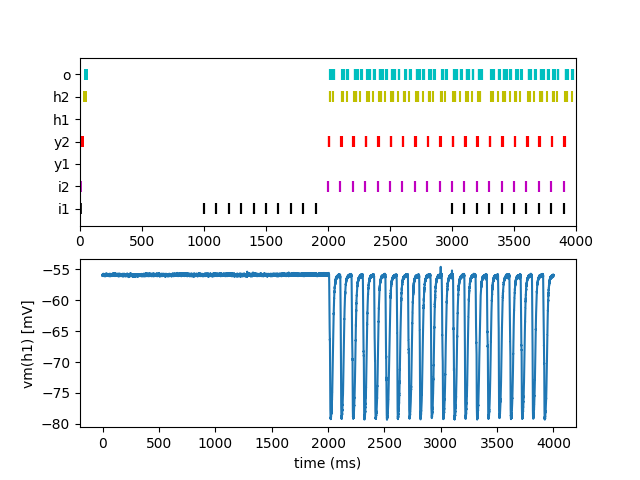
\includegraphics[scale=0.45]{pictures/aufgabe7_3.png}
\end{center}
\end{figure}


\subsection{Aufgabe 4}
What do you expect to happen if there is some jitter on the input? Check the classifi-
cation rate (correct outputs as a fraction of presented inputs) for different amounts of
jitter.

\begin{figure} [ht]
\begin{center}
\label{fig:abb4}
\caption{Feuerrate in Abhängigkeit der CVs}
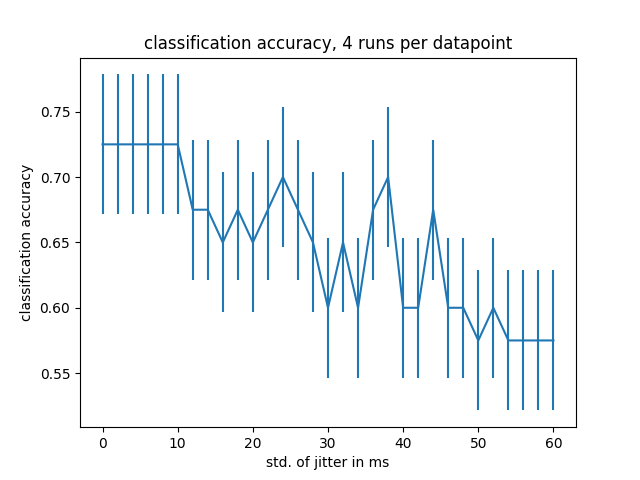
\includegraphics[scale=0.45]{pictures/jitter_plot_lang.png}
\end{center}
\end{figure}


\end{document}
